\chapter{Modal propagation in parallel plane waveguide}
	\paragraph{}
	We are investigating the propagation of electromagnetic wave inside a hollow pipe with rectangular cross section. We called this structure a rectangular waveguide. We had the structure for a rectangular waveguide shown below. With energy flowing along the length of the pipe. The coordinate axis is oriented in such direction shown with a$\geq$b.
	\begin{figure}[h]
		\centering
		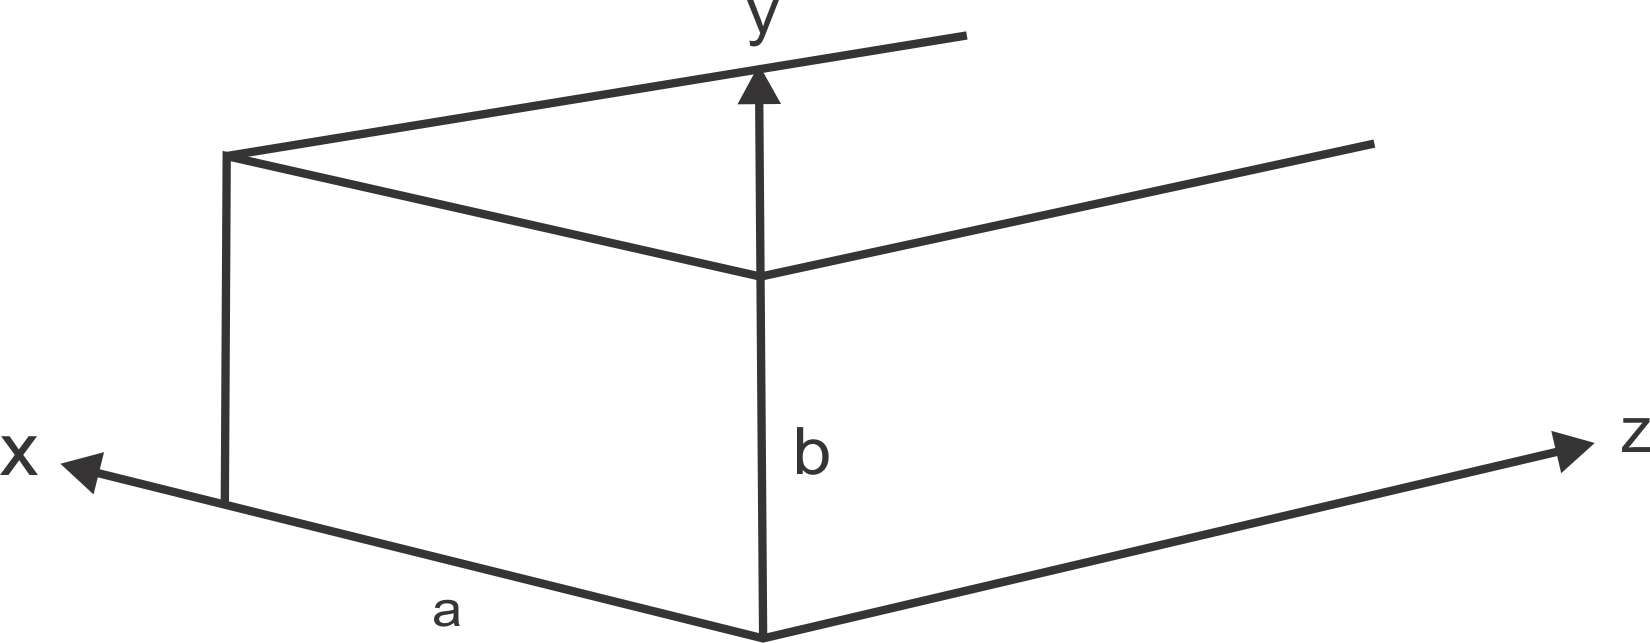
\includegraphics[width=1\linewidth]{group39}
		\caption{$a<b$}
	\end{figure}
	For the transverse electric mode, we had $E_z = 0$, $H_z \neq 0$ and by comparison we had 
	\begin{align*}
	H_z = C\cos(\frac{m\pi x}{a}) \cos(\frac{n\pi y}{b})e^{-j\beta z}
	\end{align*}
	Like the case of the transverse magnetic we denote this by $TE_{mn}$ to show the order of the transverse electric mode. We ask what are the indexes required for the existence of these fields. If $m = n = 0$ i.e $TE_{00},H_z$ is not zero unlike the $TM_{00}$ mode. Recall that the transverse fields were expressed in form below for TM modes.
	\begin{align*}
	E_x = -\frac{j\omega u}{h^2}\frac{\partial H_z}{\partial y} - \dfrac{j\beta}{h^2}\frac{\partial E_z}{\partial x}, \
	E_y = \frac{j\omega u}{h^2}\frac{\partial H_z}{\partial x} - \dfrac{j\beta}{h^2}\frac{\partial E_z}{\partial y}\\
	H_x = \frac{j\omega \epsilon}{h^2}\frac{\partial E_z}{\partial y} - \dfrac{j\beta}{h^2}\frac{\partial H_x}{\partial x}, \
	H_y = -\frac{j\omega \epsilon}{h^2}\frac{\partial E_z}{\partial x} - \dfrac{j\beta}{h^2}\frac{\partial H_z}{\partial y}
	\end{align*}
	All the transverse fields involve space derivation, $\frac{\partial}{\partial x}$ or $\frac{\partial}{\partial y}$. So having a field which does not vary as a function of space(x,y) for $TE_{00}$, $H_z = Ce^{-j\beta z}$  $\frac{\partial H_z}{\partial x}$,  $\frac{\partial H_z}{\partial y} = 0$ and $E_z = 0$ for TE. So that $E_x, E_y, H_x and H_y$ will all go to zero. So if $m = n = 0, H_z = C \Rightarrow E_\bot , H_\bot = 0$.
	This means that in this situation of $m = n = 0$ for TE, we have magnetic field $H_z = Ce^{-j\beta z}$ but no electric field. What we have seen for time varying field is such that this can't happen as electric and magnetic fields are coupled. So if electric field goes to zero, then magnetic field must go to zero. This means that the constant C is $H_z = Ce^{-j\beta z}$ must be identically be equal to zero. This means that mode $TE_{00}$ cannot exist like $TM_{00}$.
	\paragraph{}
	In $H_z = C \cos (\frac{n\pi x}{a})cu(\frac{n\pi y}{b})e^{-j\beta z}m\ or\ n\ = 0$ means the equation reduces to $H_z = C \cos (\frac{n\pi y}{b})e^{-j\beta z}$ or $H_z = C \cos (\frac{m\pi x}{a})e^{-j\beta z} \neq 0$.  That means $TE_{on}$ or $TE_{mo}$ does not exist. The $TE_{on}$ meant that the field has variation in the y-direction and mo in x-direction. $TE_{mo}$ means that the field has variation in the x-direction but no variation in the y-direction.
	\paragraph{}Hence the lowest order modes for TE mode will be $TE_{10}$ or $TE_{01}$ compared to $TM_{11}$ in 1m mode. Using similar analysis like the TM mode, it can be shown that $h^2 =(\dfrac{m\pi}{a})^2 + (\dfrac{n\pi}{b})^2$ and then we get phase constant in z-direction as $\beta = \sqrt{w^2\mu\epsilon-(\frac{m\pi}{a})^2-(\dfrac{n\pi}{b})^2}$ $\bar{E}_1\bar{H}\mu e^{-j\beta z}$ i.e $\bar{E}\ and\ \bar{H}$ has variation with $e^{-j\beta z}$ in their term to show the traveling $\omega^2\mu\epsilon < (\frac{m\pi}{a})^2 + (\dfrac{n\pi}{b})^2$, then the quantity inside the square root becomes negative and $\beta$ becomes imaginary. At this point $e^{-j\beta z}$ does not represent traveling wave, but exponentially decaying fields in the z-direction and the wave propagation cases.
	\paragraph{}Hence we see that the frequency must have certain values so that $\beta$ is a real quantity. That frequency as we saw in a parallel plane waveguide were transition takes place from wave to decaying field is the cut-off frequency of the mode. So far different values of m and n, we have different cut-off frequency. At cut-off frequency ${\omega_c}^2\mu\epsilon = (\frac{m\pi}{a})^2 + (\dfrac{n\pi}{b})^2$
	\begin{align}
	f_c = \frac{1}{2\pi \sqrt{\mu\epsilon}}((\frac{m\pi}{a})^2 + (\dfrac{n\pi}{b})^2)^{\frac{1}{2}}
	\end{align}
	Now knowing the order m and n, and the dimension of the waveguide, we can determine the cut-off frequency for a particular mode.
	\begin{align*}
	\beta = \sqrt{{\omega}^2\mu\epsilon-{\omega_c}^2\mu\epsilon},\ since\ {\omega_c}^2\mu\epsilon = (\frac{m\pi}{a})^2 + (\dfrac{n\pi}{b})^2\\
	=\omega\sqrt{\mu\epsilon}[1-{\frac{\omega c}{\omega}}]^{\frac{1}{2}} = \frac{\omega}{c} [1-{\frac{fc}{f}}]^{\frac{1}{2}} \frac{1}{\sqrt{\mu\epsilon}}=c\ so\ \omega{\sqrt{\mu\epsilon}}= \frac{\omega}{c}\\ \beta = \frac{2\pi f}{c}[1-(\frac{f_c}{f})^2]
	= \frac{2\pi}{\lambda}[1-(\frac{f_c}{f})^{\frac{1}{2}}]
	\end{align*}
	Now this is the phase constant for the waveguide in the z-direction. Now we imagine we have this structure for which the quantity we had to measure was the variation of electric field along the length, say we take a proble to measure the field along the length, you will observe a separation distance between two consecutive maximas that is related to the phase constant of the wave along the direction of the waveguide $\frac{2\pi}{\lambda}$ is what we will measure in this waveguide. This $\lambda$ is what the wave has intrinsically in an unbound medium.
	\paragraph{}For our case, let's say $\beta = \frac{2\pi}{\lambda}, \lambda$ is not wavelength in unbound medium $(\frac{c}{f})$, so we are better of saying  $\beta = \frac{2\pi}{\lambda g}$. ${\lambda g}$ best describes the distance between two maxima of electric field that we would measure inside the rectangular waveguide. So $\lambda$ is intrinsic wavelength of wave in an unbound medium $(\frac{c}{f})$, inside the wavelength we have a modified wavelength $\lambda g$ is related $\lambda$. So $\lambda g$ which is the wavelength for the guided electric and magnetic field distribution inside the rectangular waveguide, hence it is called the GUIDED WAVELENGTH, $\lambda$ is the phase constant we measured as we move the probe along to get successive maxima inside the waveguide.$\lambda$ is not what we measure along the waveguide but $\lambda g$\\
	From $\beta = \frac{2\pi}{\lambda}[1-{\frac{fc}{f}}]^{\frac{1}{2}}$ is related to  $\beta = \frac{2\pi}{\lambda g}$, then $\lambda g = \frac{\lambda}{[1-{\frac{fc}{f}}]^{\frac{1}{2}}}$ where $\lambda$ is wavelength of wave in unbound medium $\lambda g$ is the wavelength which we will measure inside the bound structure along the waveguide. For travelling wave $f>f_c$ otherwise $\lambda$ is a complex number that result to exponentially decaying fields. So $[1-{\frac{fc}{f}}]^{\frac{1}{2}}$ is always going to be less than 1. Meaning $\lambda g>\lambda$. Hence guarded wavelength is always greater than intrinsic wavelength of the medium. As $f\longrightarrow0$, $\frac{f_c}{f}\longrightarrow0$ at that time, $\lambda g\longrightarrow\lambda$ but never become $\lambda_\rho$ because we would always have a frequency which is finite. So for a guided structure, no matter what frequency we operate at $\lambda_g>\lambda$.
	\paragraph{}Secondly, as $f\longrightarrow f_c$, when $f=f_c, \lambda_g = \frac{\lambda}{0} = \infty$ so $\lambda_g\longrightarrow\infty$ when $f\longrightarrow f_c$. We know that phase velocity $V_\rho = \frac{\omega}{\beta}.\ When\\ f\gg f_c, V_\rho\approx C$ (intrinsic velocity) and when $f\longrightarrow f_c$, $V_\rho\longrightarrow\infty$ or if $\lambda_g\longrightarrow\infty$ because $f\longrightarrow f_c$, velocity = $\lambda_gf\longrightarrow\infty$.
	\paragraph{}These are certain important conclusions we can draw for the wave we came bode to the field expression and try to investigate the cut-off frequencies for different modes. Comparing the\\ lowest modes for the TE and TM mode, which are $TE_{10}, TE_{0}1,\ and\ TM_{11}$.
	\begin{align*}
	f_c = \frac{1}{2\pi \sqrt{\mu\epsilon}}[(\frac{m\pi}{a})^2 + (\dfrac{n\pi}{b})^2]^{\frac{1}{2}}\ for\ m=1\ and\ n=0\\
	TE_{10}\ have\ f_c = \frac{1}{2\pi \sqrt{\mu\epsilon}}\frac{\pi}{a},\ for\ m=0\ and\ n=1\ f_c = \frac{1}{2\pi \sqrt{\mu\epsilon}}\frac{\pi}{b}\\
	for\ TM_{11},\ f_c = \frac{1}{2\pi \sqrt{\mu\epsilon}}[(\frac{\pi}{a})^2 + (\dfrac{\pi}{b})^2]^{\frac{1}{2}}\\
	f_{cTE_{10}} = \frac{\frac{\pi}{a}}{2\pi \sqrt{\mu\epsilon}}, f_{cTE{01}} = \frac{\frac{\pi}{a}}{2\pi \sqrt{\mu\epsilon}}, f_{cTM{11}} = \frac{[(\frac{\pi}{b})^2 + (\dfrac{\pi}{b})^2]^{\frac{1}{2}}}{2\pi \sqrt{\mu\epsilon}}
	\end{align*}
	Recall by definition that a>b, for a square waveguide a=b. For a rectangular waveguide with a>b, $f_{cTE{10}}$ is less than $f_{cTE{01}}$ and they are both smaller than $f_{cTM{11}}$. So in general, the three lowest mode for TE and TM have $f_{cTE{10}}<f_{cTE{01}}<f_{cTM{11}}$. As we have seen $TE_{00}\ or\ TM_{00}$ do not exist so $f_{cTE{10}}$ is the lowest frequency which can propagate on the rectangular waveguide structure. That is the absolute minimum frequency which the structure will support so whenever we try to excite a rectangular waveguide, the possibility of exciting the $TE_{10}$ mode is highest, because if the wave is going to propagate at all, it will be propagating in the frequency around $f_{cTE{10}}$. If the frequency lies between $f_{cTE{10}}\ and\ f_{cTE{01}}$, it is likely $TE{10}$ will propagate. If it lies within $f_{cTE{01}}\ and\ f_{cTM{11}}$, it is possible $f_{cTE{10}}\ and\ f_{cTE{01}}$ will propagate and $f_{cTM{11}}$ will not propagate. $f_{cTE{10}}$ is the lowest frequency which the waveguide is capable of supporting. This is the reason the $TE_{10}$ mode is called the DOMINANT MODE of a rectangular waveguide, $TE_{10}$ mode means there is one half cycle variation in the x-axis and no variation on the y-axis. Since it is the dominant mode, we can have a detailed analysis of this mode rather than talking about the general mode of $TE_{mn}$ or $TM_{mn}$, since if at all energy is going to propagate, it is going to be propagated in this mode depending upon the value of a and b. It is possible that the $TE_{01}$ mode may have a frequency lower than or higher than $TE_{20}$ mode or $TE_{30}$ mode lower than the $TE_{11}$ mode or $TM_{11}$ mode. So depending upon the dimension, the ratio of a and b, it is possible that a higher order TE mode like $TE_{20}$ or $TE_{30}$ may have a cut-off frequency smaller than $TM_{11}$ or they may have frequency more than that. So one cannot make a general statement about what is the order of the cut-off frequency for the various modes of $TE_{mn}\ or\ TM_{mn}$. However, certain things are true here, the lowest frequency is always $TE_{10}$ mode, for this reason, if we wanted to have a single mode operation inside the waveguide, the energy always propagates in the dominant mode called the electric field for $TE_{10}$ modes, we get $H_z$, substitute m=1, n=0 in $H_z = C \cos (\frac{m\pi x}{a})\cos(\frac{n\pi y}{b})e^{-j\beta z}$, substitute into the transverse fields expression, we get the remaining components for the $TE_{10}$ modes. So for this case
	\begin{dmath*}
	H_z = C\cos(\frac{\pi x}{a})e^{-j\beta z},\ H_z\ is\ only\ a\ function\ of\ x, \Rightarrow \frac{\partial}{\partial y} = 0, so\\
	E_x = \frac{-j\omega\mu}{h^2}\frac{\partial H_z}{\partial y} - \dfrac{j\beta}{h^2}\frac{\partial E_z}{\partial x}, E_z = 0\ for\ TE\ case\ therefore\ E_x = 0,\\
	E_y = \frac{j\omega\mu}{h^2}\frac{\partial H_z}{\partial x} - 
	\frac{j\beta}{h^2}\frac{\partial E_z}{\partial y}, 
	\frac{j\omega\mu}{(\frac{\pi}{a})^2} - C(\frac{\pi}{a})\sin(\frac{\pi x}{a})e^{-j\beta z},\\
	H_x = \frac{j\omega\epsilon}{h^2}\frac{\partial E_z}{\partial y} - 
	\frac{j\beta}{h^2}\frac{\partial H_z}{\partial x}, 0 - \frac{j\beta}{(\frac{\pi}{a})^2} - C(\frac{\pi}{a})\sin(\frac{\pi x}{a})e^{-j\beta z},\\
	H_y = \frac{-j\omega\epsilon}{h^2}\frac{\partial E_z}{\partial x} - 
	\frac{j\beta}{h^2}\frac{\partial H_z}{\partial y}, E_z = 0 \frac{\partial H_z}{\partial y} = 0\ therefore\ H_y = 0\\
	recall\ h^2 =(\dfrac{m\pi}{a})^2 + (\dfrac{n\pi}{b})^2 m = 1, h = \frac{\pi}{a}\ for\ TE_{10}
	\end{dmath*}
	\paragraph{}In summary for the $TE_{10}$ mode, we have $H_z = C\cos(\frac{\pi x}{a})e^{-j\beta z}, E_x = 0, H_y = 0, h = \frac{\pi}{a}, E_y = 	\frac{-j\omega\mu }{(\frac{\pi}{a})^2}C(\frac{\pi}{a})\sin(\frac{\pi x}{a})e^{-j\beta z}, H_x \frac{j\beta}{(\frac{\pi}{a})^2}C(\frac{\pi}{a})\sin(\frac{\pi x}{a})e^{-j\beta z}.$ So $TE_{10}$ mode has only one electric field component in the y-direction $E_y$ and two magnetic field components $H_x\ and\ H_z$. $E_x, E_z = 0, E_y = \frac{-j\omega\mu a}{\pi}C\sin(\frac{\pi x}{a})e^{-j\beta z}, H_x = \frac{-j\beta a}{\pi}C\sin(\frac{\pi x}{a})e^{-j\beta z}.\\ H_y = 0\ and\ H_z = C\cos(\frac{\pi x}{a})e^{-j\beta z}.$ These are the expressions for the fields of a dominant waveguide and normally we operate the waveguide in this mode. Many times we have a requirement that there should be single mode propagation on the rectangular waveguide and the simple mode propagation will take place in the dominant mode. These are the fields that will exist in the waveguide in this single mode of propagation, we substitute into the expression for the wavelength to get the cut-off wavelength and then calculate the phase constant associated with the wavelength. Looking at the appearance of the $TE_{10}$ mode field, we have electric field being y-oriented. Hence we get a maximum electric field at the centre all pointed in the y-direction.
	\begin{figure}[h]
		\centering
		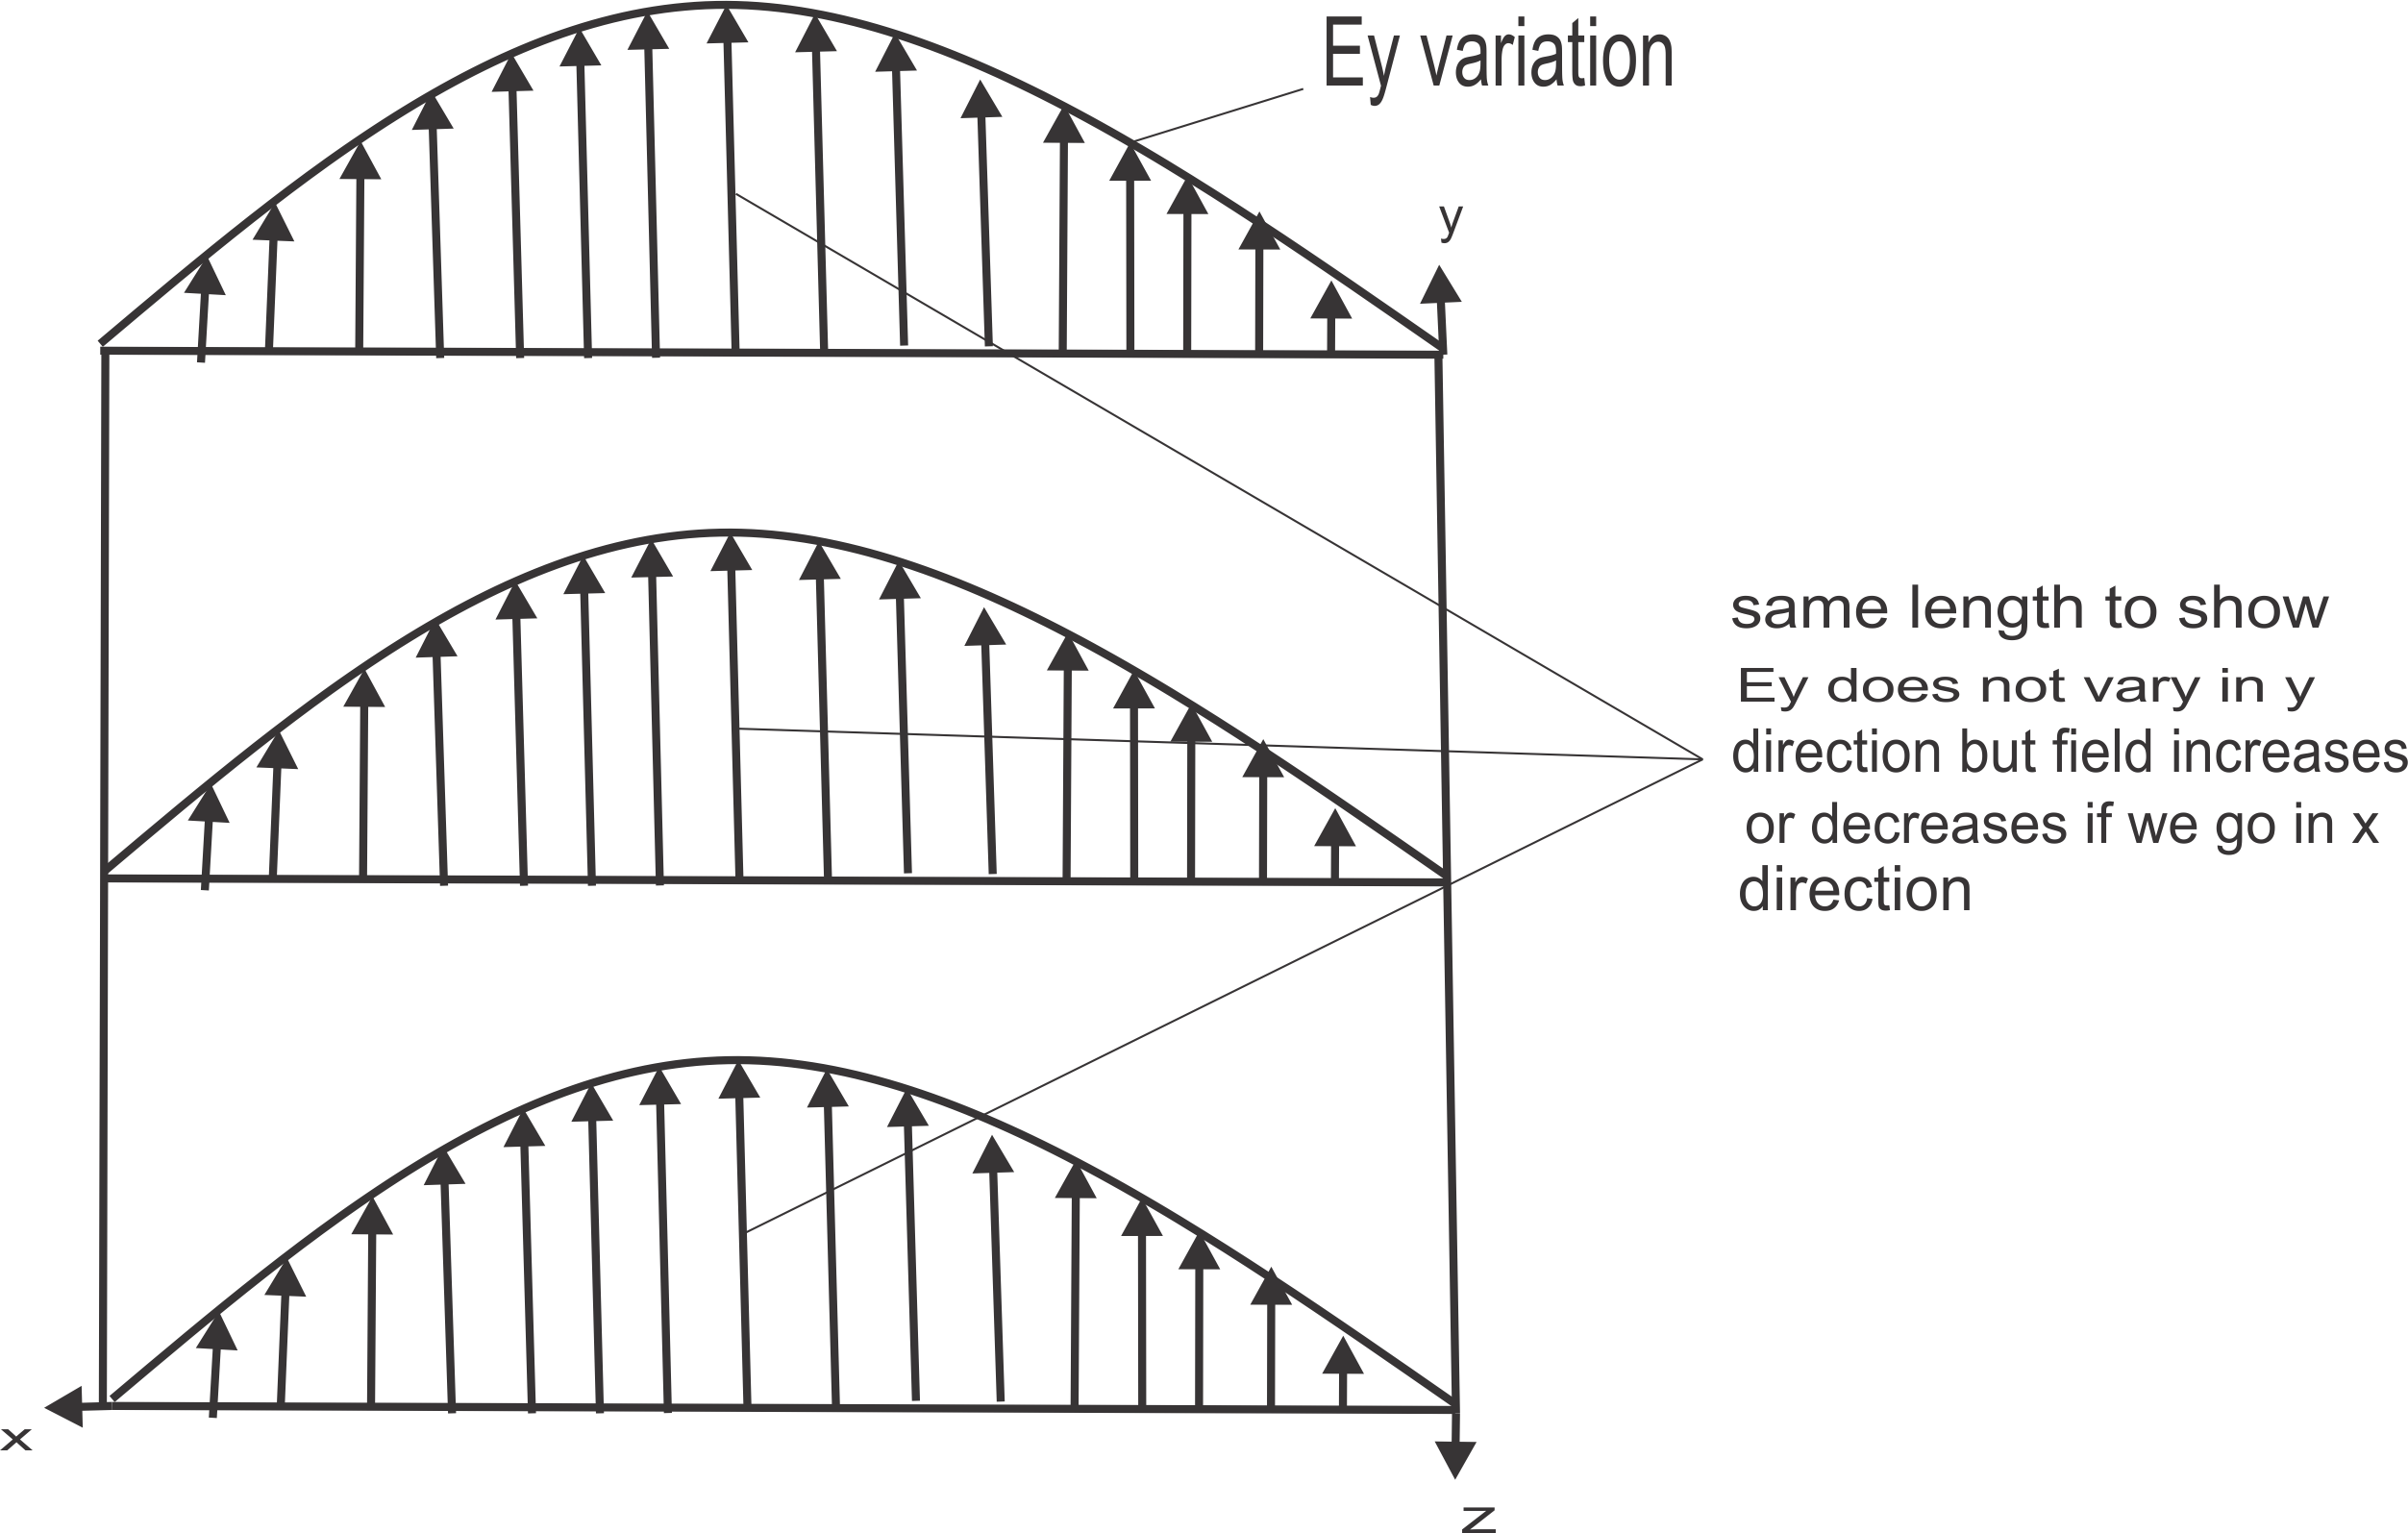
\includegraphics[width=1\linewidth]{group39-1}
		\caption{}
	\end{figure}
	 The field at a y-location is the same in magnitude and direction. However, it varies as we move in the x-direction, maximum at x = o and at x = a. The tangential components of $E_y$ against the side walls is equal to zero, we visualize the detail of these fields in different waveguiding structure later. At the moment, it appears $E_y$ is maximum at the broader wall of the waveguide as shown by the line traced on the waveguide. Same thing will happen to higher modes also you find the locations were the electric and magnetic fields are maximum. Why this information is important is one can ask a question that a waveguide is giving to you. How can a particular mode be excited inside the waveguide? Do we have a mechanism by which a particular order mode can be excited or cam we selectively excite certain mode inside a waveguide?
	 	\begin{figure}[h]
	 	\centering
	 	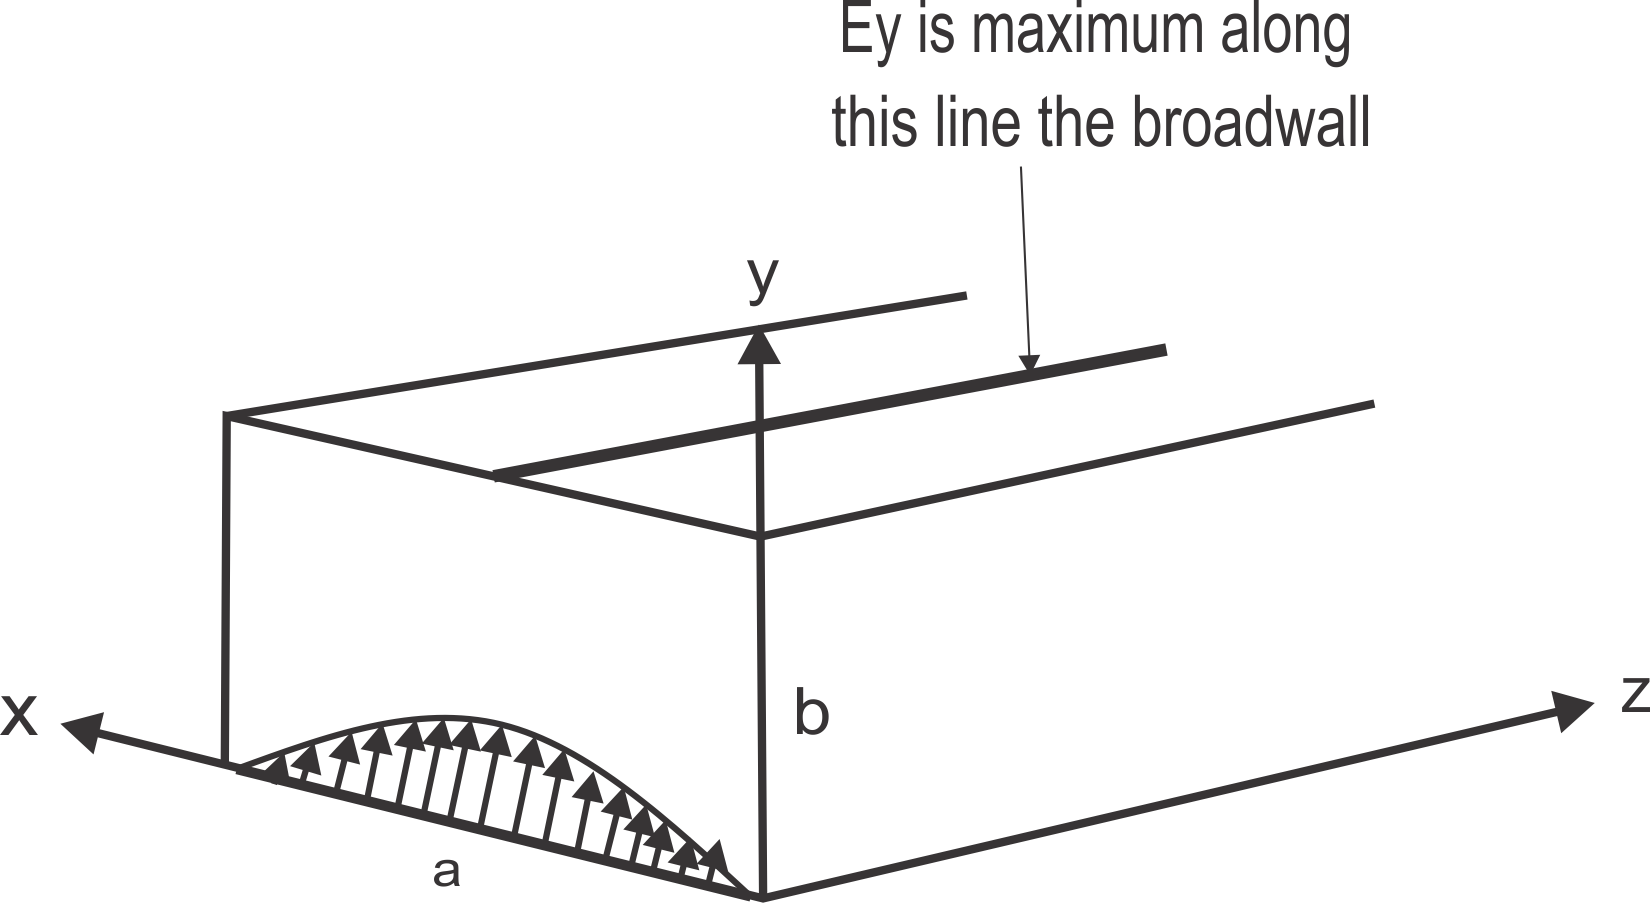
\includegraphics[width=1\linewidth]{group39-2}
	 	\caption{}
	 \end{figure}
	  By looking at the field distribution, it becomes clear that yes, if we create a mechanism by which the field is maximum along the line shown above and as such the mode which will be excited inside the waveguide will be the $TE_{10}$ mode. So two things are required for excitation of this $TE_{10}$ mode, first the size of the waveguide should be such that the frequency. Secondly, the excitation mechanism should be such that the field or mode which we want to get excited, match with the excitation i.e maximum at the broader wall for the $TE_{10}$ mode in this case. So for the excitation of the $TE_{10}$ mode, we put some kind of a probe inside the waveguide on the broad wall and because of that we have a finite field. For $TE_{10}$ mode, we talked about the field distribution satisfies the boundary conditions. We have the point of field excitation as shown below, then we show that to satisfy the boundary condition for a field, we require all possible modes for the waveguide either for traveling or decaying.
	  	\begin{figure}[h]
	  	\centering
	  	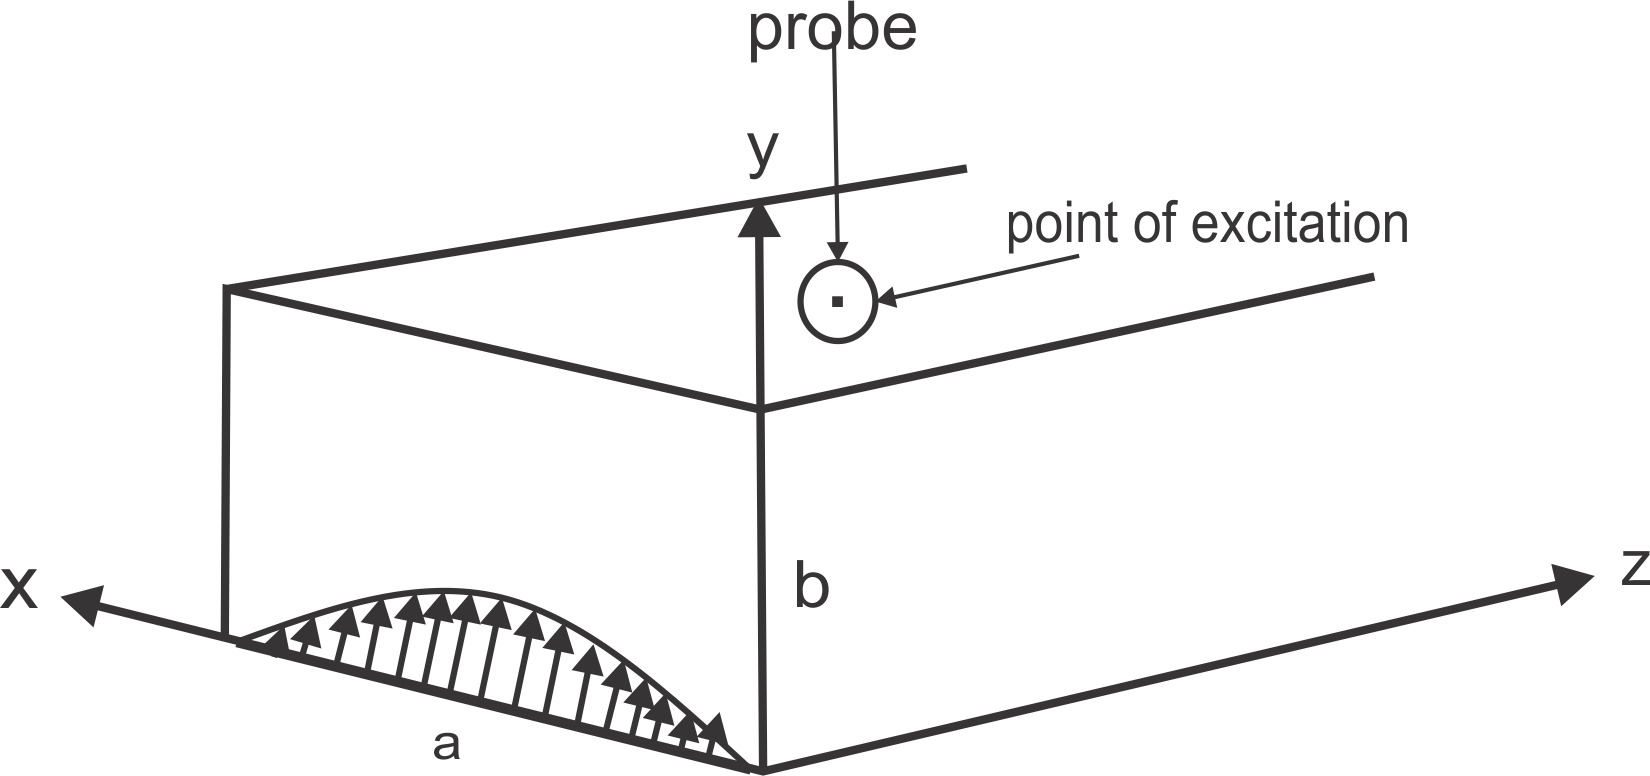
\includegraphics[width=1\linewidth]{group39-3}
	  	\caption{}
	  \end{figure}
	  These are essentially three orthogonal functions which satisfy the boundary condition inside the x structure. So locally around the probe all kinds of modes gets excited inside the waveguide, including the fields which are decaying fields. Only as we travel further in the waveguide, those fields which are below cut-off will die down rapidly only that frequency for which the cut-off frequency is less than this will travel. If we make sure that this frequency is larger than the cut-off frequency of the $TE_{10}$ mode but smaller than any of the other cut-off frequencies, we get the $TE_{10}$ mode inside the waveguide structure guaranteed. So essentially a $TE_{10}$ mode inside the waveguide can be excited by pulling a probe which can excite electric field inside the waveguide at the middle of the broader wall.
	  \paragraph{}In practice, whenever we do the experiment, or we carry the high frequency signals like microwave signals, these signals are carried by a rectangular waveguide and this rectangular waveguide always operate in  a mode which is the dominant mode of the waveguide called the $TE_{10}$ mode.
	  \paragraph{}One can ask the question, how do we get the saying that we should operate this waveguide in a single mode operation. These are many application were we want single mode operation. The question is why do we want single mode operation. The answer essentially lies in our dispersion relation. It says that the phase constant is a function of m and n i.e $\beta = \sqrt{{\omega}^2\mu\epsilon - (\frac{m\pi}{a})^2 - (\frac{n\pi}{b})^2}.$ Hence the velocity of the mode is a function of m and n. This means that for a given frequency $\omega$, the different modes are going to travel with different speeds. Now to send information on this waveguide, we try to put energy inside this waveguiding structure and then if larger modes can be supported by the waveguide structure, if the waveguide is not in single mode operation, the energy will get distributed into various modes i.e various combinations of m and n. Each mode will have its own velocity for traveling. So as it travels, the energy which is going on different modes is essentially separated. Imagine a situation were we transmit signals which are not time varying sinusoidal signals, say a pulse at high frequency, now if the energy is divided into different modes, and different modes travel at different speeds, than the energy reaches the other side of the waveguide, then all the modes will not reach the other end at the same time. That means the energy packet we send, will not be the energy packet we receive as they will be distributed in time as some modes will arrive earlier, some modes will arrive later. So the dispersion phenomena we talk about essentially will give us the broadening of the signal in time as it travels on the waveguide. This is happening because energy is being distributed into various modes and different modes travel at different speed. To avoid this, we try to put the energy only in one mode so that energy remains in that mode, so that the distribution of energy or differential delays which can be caused because of multiple mode of propagation inside the waveguide is avoided and we do not have broadening of the signal when it travels on the waveguide, because of multi mode propagation. This is the aspect one is to make use of when we design the waveguides at high frequencies.
	  \paragraph{}In conclusion, for a rectangular waveguide, the important mode is the transverse electric mode $TE_{10}$ mode, that mode we also call DOMINANT MODE because it has the lowest cut-off frequency and for this frequency, we should make sure single mode propagation takes place over certain range of frequencies. So in experiments, we make sure the frequency lies in that range so there is a single mode propagation.
  